\documentclass[conference]{IEEEtran}
\IEEEoverridecommandlockouts
% The preceding line is only needed to identify funding in the first footnote. If that is unneeded, please comment it out.
%Template version as of 6/27/2024

\usepackage{cite}
\usepackage{amsmath,amssymb,amsfonts}
\usepackage{algorithmic}
\usepackage{graphicx}
\usepackage{textcomp}
\usepackage{xcolor}

\usepackage{booktabs}
\usepackage{siunitx}
\sisetup{output-decimal-marker = {,}}


\usepackage{booktabs}   % Para \toprule, \midrule, \bottomrule
\usepackage{siunitx}
\sisetup{group-separator = {\,}, group-minimum-digits=4}
% Para o alinhamento de números na coluna S
\usepackage{multirow}   % Para mesclar linhas com \multirow
\usepackage{graphicx}   % Para o comando \resizebox

% --- AJUSTES DE TEXTO ---
\usepackage{hyphenat}
\hyphenation{Res-Net}
\sloppy
\def\BibTeX{{\rm B\kern-.05em{\sc i\kern-.025em b}\kern-.08em
    T\kern-.1667em\lower.7ex\hbox{E}\kern-.125emX}}
\begin{document}
\title{MLBFA: A Machine Learning-Guided Framework for Efficient Bit-Flip Attacks on Deep Neural Networks\\
{\footnotesize \textsuperscript{*}}
\thanks{This project was supported by the Ministry of Science, Technology and Innovations, with resources from Law No. 8,248 of October 23, 1991, under the PPI-SOFTEX program, coordinated by Softex, and published as ‘Residência em TIC 37’ (DOU 01245.001849/2024-76).}
}

\author{\IEEEauthorblockN{1\textsuperscript{st} José Ronaldo}
\IEEEauthorblockA{\textit{Laboratório de Sistemas Digitais (LSD)} \\
\textit{Federal Institute of Ceará, Maracanaú}\\
Maracanaú, Brasil \\
ronaldoferrreira.b@gmail.com}
\and
\IEEEauthorblockN{2\textsuperscript{nd} Otávio Alcântara de Lima}
\IEEEauthorblockA{\textit{Laboratório de Sistemas Digitais (LSD)} \\
\textit{Federal Institute of Ceará, Maracanaú}\\
Maracanaú, Brasil\\
otavio@ifce.edu.br }
\and
\IEEEauthorblockN{3\textsuperscript{rd} Nayra Sousa}
\IEEEauthorblockA{\textit{Laboratório de Sistemas Digitais (LSD)} \\
\textit{Federal Institute of Ceará, Maracanaú}\\
Maracanaú, Brasil\\
nayra.sousa07@aluno.ifce.edu.br}

}


\maketitle

\begin{abstract}
The deployment of Deep Neural Networks (DNNs) in safety-critical systems requires resilience against hardware-level threats such as Bit-Flip Attacks (BFAs), including those enabled by memory fault mechanisms (e.g., RowHammer). This challenge is particularly relevant for quantized models, which are generally more robust than floating-point networks and therefore demand more sophisticated strategies to identify minimal critical fault patterns. This paper introduces MLBFA, a machine-learning-guided framework for efficient BFAs on quantized DNNs. MLBFA follows a three-stage methodology: (i) it trains a Vulnerability Model (VM) from a limited statistical fault injection campaign using a multidimensional feature set; (ii) it applies the VM to generate a full-network vulnerability ranking; and (iii) it exploits this ranking to guide different search algorithms (Greedy, Evolutionary, and Progressive) toward compact sets of bit-flips that degrade the network below a target accuracy. Experimental results on quantized ResNet architectures show that MLBFA substantially reduces the number of required bit-flips compared to gradient-based baselines. In particular, the pruning-enhanced variant (MLBFA-Pruned) compromises an 8-bit ResNet-56 with five flips (a 50\% reduction compared to the baseline MLBFA configuration without pruning) and achieves five flips versus sixteen reported by the state of the art. Moreover, a regression-based vulnerability ranking is found to be less efficient and less stable than the classification-based VM, supporting the use of binary vulnerability modeling for attack optimization. Overall, the results indicate that ML-guided vulnerability maps provide an effective mechanism for accelerating and strengthening hardware-induced attacks under constrained fault budgets.
\end{abstract}


\begin{IEEEkeywords}
Deep Neural Networks, Bit-Flip Attack, Fault Injection, Machine Learning, Vulnerability Model, Hardware Security, Reliability.
\end{IEEEkeywords}

% --- INTRODUÇÃO ---
\section{Introduction}
\label{sec:introducao}

As Deep Neural Networks (DNNs) are increasingly deployed in safety-critical applications, such as autonomous vehicles and medical diagnostics, their reliability has become a paramount concern. The integrity of these models is threatened by a spectrum of issues, ranging from physical hardware faults (e.g., silicon aging and radiation-induced upsets) to direct malicious attacks~\cite{Lin, indi}. Among these threats, Bit-Flip Attacks (BFAs) stand out due to their stealthy and high-impact nature~\cite{Qian2023}. A prominent physical exploit capable of inducing BFAs is RowHammer~\cite{Kim2014,BREIER2023}, where repeated accesses to adjacent memory rows corrupt stored DNN weights, silently degrading inference quality. Consequently, assessing and understanding the robustness of DNNs against such faults has become a critical research frontier~\cite{bosio2019, ruospo2020, Ahmadilivani2024, Liu2017, sabbagh2019evaluating, Qian2023, Torres, Yu}.

The standard approach for evaluating resilience is software-based Fault Injection (FI), which offers low cost and high controllability~\cite{Arlat1990, Ruospo2021, Ruospo2023}. Widely adopted frameworks, such as PyTorchFI, TensorFI, and Multi-Resolution Fault Injection (MRFI), provide practical means to emulate faults and quantify their impact~\cite{Mahmoudetal2020, chen2018tensorfi, Huang2023MRFI, Gavarini2023, Zheng2023, agarwal_lltfi_2021, reagen2018ares, Gogebakan}. However, for modern DNNs with millions of parameters, exhaustive FI campaigns that test every possible bit-flip remain computationally infeasible, making the systematic identification of critical vulnerabilities a formidable challenge~\cite{salih2022survey, ruospo2023assessing, Gavarini2023, Zhang2022, Zhang2023}.

To manage this complexity, prior work has largely diverged into two complementary research directions: vulnerability modeling for defense and heuristic-guided search for attacks. On the defense side, Statistical Fault Injection (SFI) provides global reliability estimates but typically lacks the granularity needed to pinpoint specific weak parameters for selective hardening~\cite{ruospo2023assessing, ruospo2025iterative, leveugle2009statistical}. More recently, machine-learning vulnerability models have shown that a small FI sample can be leveraged to predict the vulnerability of all model parameters, enabling targeted protection mechanisms~\cite{Zhang2022, Zhang2023, Traiola2023hardnning, harDNNing2023, Huang2020Functional}. In contrast, state-of-the-art BFA methods still rely mostly on simpler, single-metric heuristics—commonly gradients or saliency—combined with search procedures such as Progressive Bit Search (PBS)~\cite{Rakin2019, Rakin2021, Hector2022, Dong}. This reveals a methodological gap: while multidimensional vulnerability modeling has matured in the context of reliability and defense, attack strategies have not yet systematically leveraged such models to guide their search for critical bit patterns.

This work addresses this gap by introducing MLBFA, a framework that uses a machine-learning-based Vulnerability Model (VM) to guide efficient bit-flip attacks on quantized DNNs. Quantized networks are the focus of this study because they are generally more robust than floating-point counterparts, in which isolated flips can be catastrophic~\cite{Rakin2019}. At the same time, this robustness makes the discovery of minimal fault patterns considerably more challenging, motivating the use of richer vulnerability characterization beyond conventional heuristics. The proposed methodology follows a three-stage process: (i)~a predictive VM is trained from a limited SFI campaign using 21 predictors grouped into three categories:
intrinsic/architectural (8): weight magnitude/sign, layer and parameter index, layer sparsity, and convolutional hyperparameters (stride, dilation, groups);
data-driven (7): gradient-based sensitivity, reuse count, Hessian-diagonal proxy, input/output channel energy, and saliency scores (SNIP, SynFlow);
and log-/logit-transformed variants (6): variance-stabilized transforms of influence, energies, sparsity, and saliencies (e.g., influence log, $E_{\text{in/out}}$ logs, sparsity logit, SNIP/SynFlow logs).
(ii)~the VM is then used to construct a full-network vulnerability map that ranks parameters by predicted fault criticality; and (iii)~this ranking guides different search strategies (Greedy, Evolutionary, and PBS) to identify small sets of bit-flips that degrade the model below a target accuracy.

To improve attack efficiency, we incorporate a pruning mechanism into the guided search (MLBFA-Pruned), which reduces the candidate space and lowers the number of required bit-flips in most settings. MLBFA-Pruned improves or matches the baseline in 11 out of 12 configurations, achieving its largest gains in deeper networks; for example, on 8-bit ResNet-56 it reduces the attack cost from 10 to 5 flips (50\%). Compared to the state of the art by Rakin et al.~\cite{Rakin2019}, our method further decreases the flip budget, requiring 5 flips on 8-bit ResNet-56 versus 16 in the baseline. These results are supported by repeated trials (up to 24 runs per configuration), enabling a statistical assessment of efficiency and reproducibility.

We also evaluate a regression-based vulnerability ranking strategy, in which the VM predicts the degradation magnitude rather than a binary vulnerability label. This formulation is consistently less effective, requiring substantially more flips (e.g., 10 versus 4 on ResNet-32) and exhibiting lower stability in deeper models (e.g., 36 versus 8 on ResNet-44), indicating that classification provides a more reliable guidance signal for minimizing fault sets.

The remainder of this paper is organized as follows. Section~\ref{sec:framework} presents the MLBFA framework. Section~\ref{sec:results} details the experimental setup and results. Finally, Section~\ref{sec:conclusions} concludes the paper and discusses future directions.













\section{Background}
\label{sec:background}

\subsection{Statistical Fault Injection (SFI)}
SFI models fault injection as random sampling without replacement from a finite population of $N$ faults~\cite{leveugle2009statistical}. To estimate the true failure rate $p$ with a margin of error $\varepsilon$ and confidence level $1-\alpha$, the required sample size $n$ is derived using the Finite Population Correction (FPC)~\cite{leveugle2009statistical}:
\begin{equation}
n = \frac{N\,t_{1-\alpha/2}^2\,p(1-p)}{\varepsilon^2 (N-1) + t_{1-\alpha/2}^2\,p(1-p)},
\label{eq:n_fpc}
\end{equation}
where $t_{1-\alpha/2}$ is the standard normal quantile (e.g., $2.576$ for 99\% confidence). We evaluate four paradigms classified into two categories:

\subsubsection{Data-Aware One-Step SFI}
Targeting 8-bit quantized weights, the \textit{BIT-ONE} paradigm exploits the intuition that bit-flips in different positions cause varying impact magnitude. Inspired by~\cite{ruospo2023assessing}, we define a weighted average distance $D_{\text{avg}}(i,\ell)$ for bit-plane $i$ in layer $\ell$, which captures the structural impact of a fault. This metric is mapped to a proxy probability $p(i,\ell)$ via min-max normalization to $[0, 0.5]$:
\begin{equation}
p(i,\ell) = a + \frac{(D_{\text{avg}}(i,\ell) - D_{\min})(b-a)}{D_{\max} - D_{\min}}.
\label{eq:p_data_aware}
\end{equation}
Bits causing larger perturbations receive $p(i,\ell)$ closer to $0.5$, increasing the sample size via Eq.~\eqref{eq:n_fpc}. The campaign samples $n(i,\ell)$ faults independently per bit-plane in a single step.

\subsubsection{Iterative SFI Paradigms}
Iterative campaigns refine the sample size $n_k$ dynamically based on the observed failure rate $\hat{p}_k$ after $k$ iterations~\cite{ruospo2025iterative}. To accelerate convergence, we employ the "E--P curve" methodology, which adjusts the target margin $\varepsilon_{\text{next}}$ based on $\hat{p}_k$ using a quadratic function $\varepsilon_{\text{poly}}(\hat{p})$ clipped to $\varepsilon_{\text{goal}}$ and the current margin $\hat{\varepsilon}_k$:
\begin{equation}
\varepsilon_{\text{next}} = \max\left\{\varepsilon_{\text{goal}}, \; \min\left\{\varepsilon_{\text{poly}}(\hat{p}_k), \; \frac{\hat{\varepsilon}_k}{3}\right\}\right\}.
\label{eq:ep_next}
\end{equation}
The updated sample size $n_{k+1}$ is calculated by substituting $p=\hat{p}_k$ and $\varepsilon=\varepsilon_{\text{next}}$ into Eq.~\eqref{eq:n_fpc}. We implement this mechanism across three granularities:

\begin{itemize}
    \item \textit{BIT-ITER}: Applies the iterative loop to each bit-plane $i$ independently, refining $n$ based on the specific failure rate of that bit position.
    \item \textit{LAYER}: Treats each network layer as a distinct population. The iterative convergence is enforced strictly per layer, ensuring statistical significance for local sensitivity analysis
    \item \textit{NET}: Treats the entire network as a single global population of faults. This paradigm offers the fastest convergence for global failure rate estimation but lacks granularity
\end{itemize}



\section{Proposed Framework}
\label{sec:framework}




We propose a MLBFA designed to compromise a Deep Neural Network (DNN) with a minimal number of bit-flips. The framework, illustrated in Figure~\ref{fig:framework_diagram}, operates in three stages: (1) building a VM to identify susceptible DNN weights; (2) using the VM to predict and rank the vulnerability of all weights; and (3) employing a search algorithm to find the smallest set of bit-flips that degrades accuracy to a random-guess state. Our search process utilizes not only the classic Progressive Bit Search (PBS)~\cite{Rakin2019, Rakin2021} but also novel greedy and evolutionary algorithms. The attack is untargeted and white-box, assuming full access to the DNN's parameters~\cite{Qian2023}. We focus exclusively on 4, 6, and 8-bit quantized DNNs, as they are more robust than their floating-point counterparts in which single flips can be catastrophic~\cite{Rakin2019}.

\begin{figure}[ht]
    \centering
    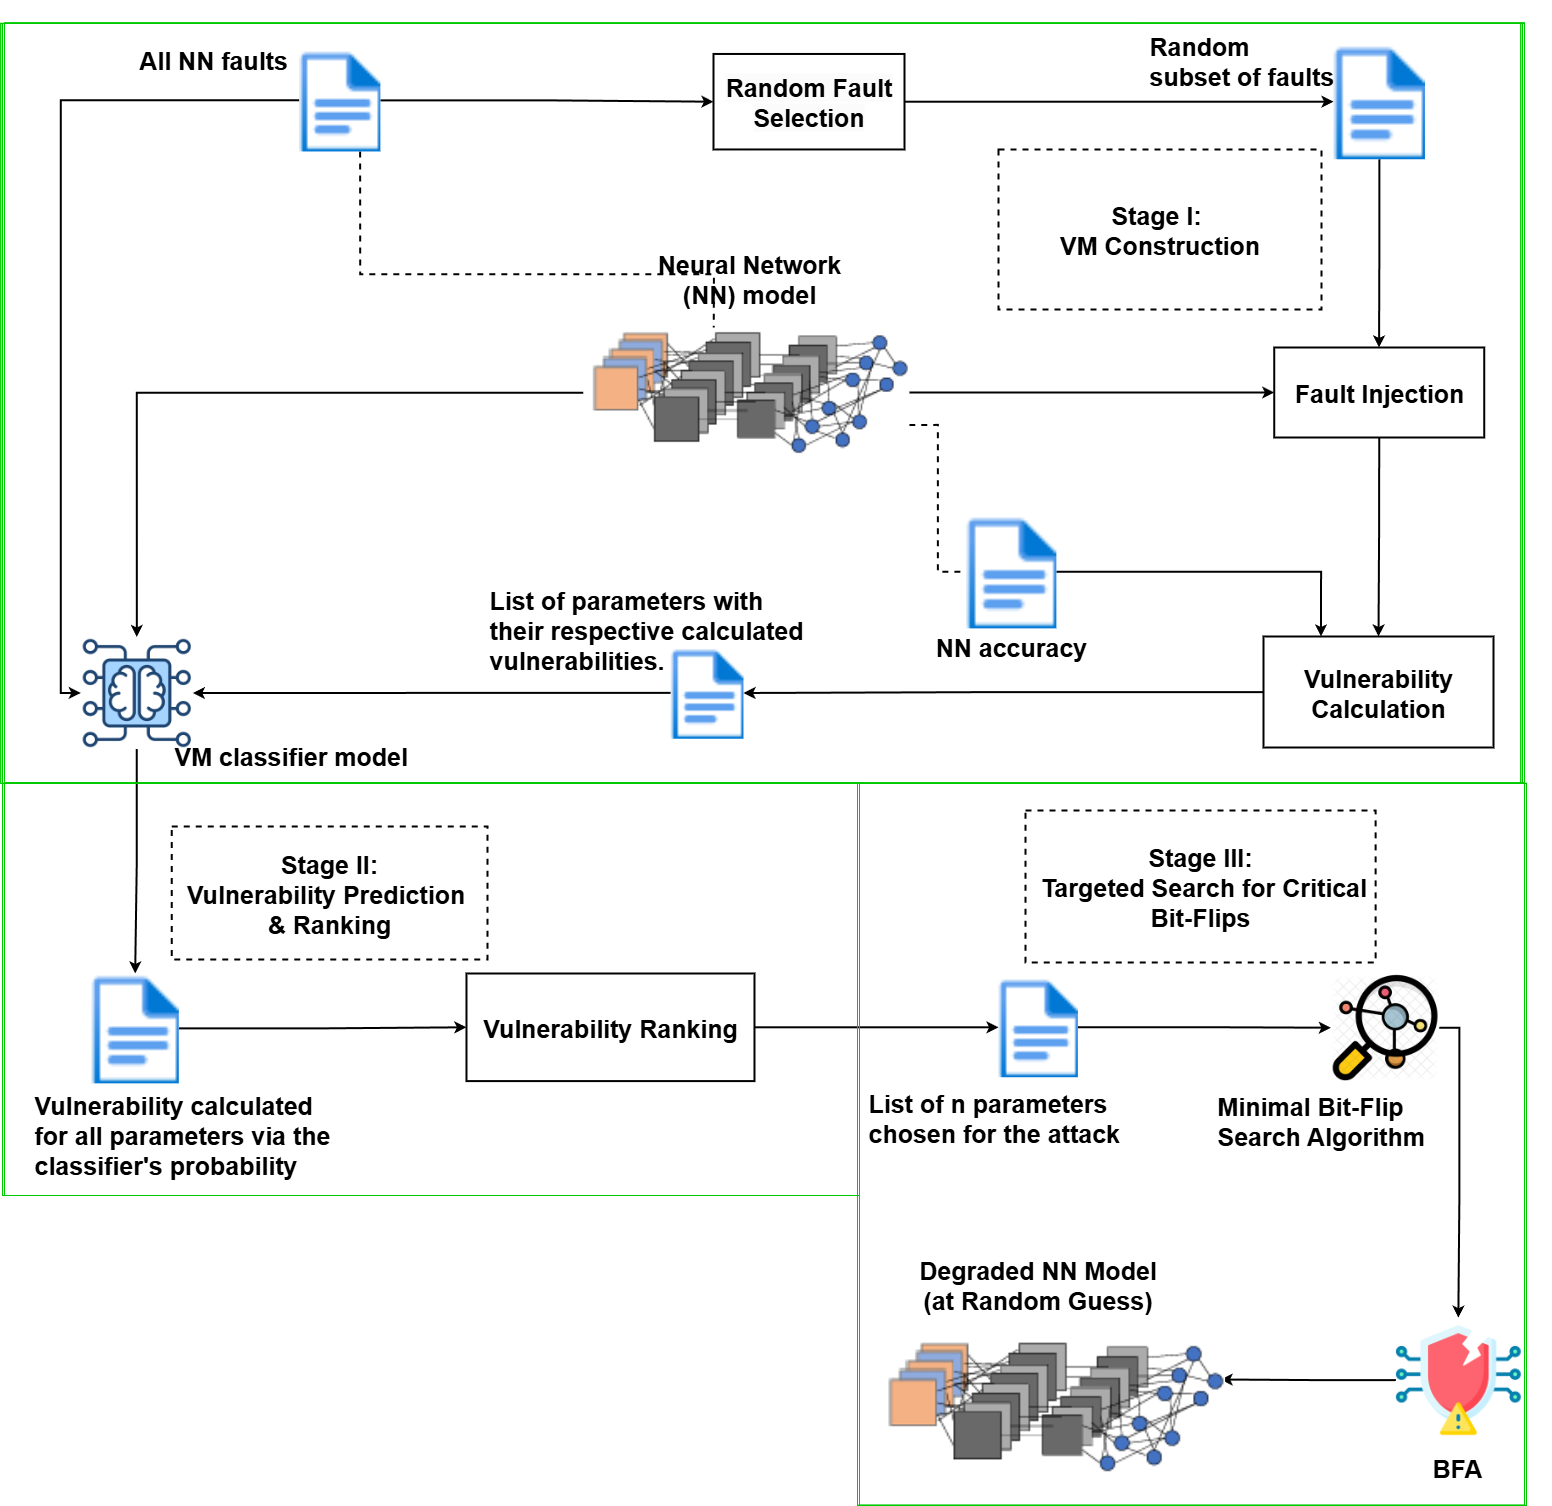
\includegraphics[width=1.03\columnwidth]{ultima.png} 
    \caption{Overview of the MLBFA methodology, detailing the three core stages: VM Construction, Vulnerability Prediction \& Ranking, and Targeted Search for Critical Bit-Flips}
    \label{fig:framework_diagram}
\end{figure}

\paragraph{Stage I: VM Construction}
The core of our framework is the VM, a machine learning model designed to predict fault susceptibility without the prohibitive cost of exhaustive injection~\cite{harDNNing2023, Gavarini2023, Ruospo2023}. Unlike previous works that rely on a single sampling strategy, we leverage the four SFI paradigms defined in Section~\ref{sec:background} (\textit{BIT-ONE}, \textit{BIT-ITER}, \textit{LAYER}, and \textit{NET}) to generate diverse training datasets. This allows us to evaluate how data granularity influences the VM's predictive power.

For each SFI paradigm, the sample size $n$ is determined by either Eq.~\eqref{eq:n_fpc} or Eq.~\eqref{eq:p_data_aware}, ensuring statistical significance with a 99\% confidence level. Each injected fault is evaluated on a subset of $K$ validation samples (where $K \in \{1024, 2048, 10000\}$), mapping the perturbed parameter to its impact on network accuracy. From this data, we train two types of VMs using an Extra Trees algorithm: (i) a \textbf{classifier}, which predicts a binary vulnerability label based on an accuracy drop threshold, and (ii) a \textbf{regressor}, which predicts the continuous magnitude of the accuracy degradation.

To capture the complex non-linear behavior of faults, each instance in the dataset is enriched with a comprehensive 21-predictor feature vector, extending the work of Zhang et al.~\cite{Zhang2022,Zhang2023}:
\begin{itemize}
  \item \textit{Intrinsic \& Architectural (8):} weight magnitude/sign, layer depth, parameter index, sparsity, and convolutional hyperparameters (stride, dilation, groups).
  \item \textit{Data-driven (7):} gradient magnitude (mean $|\partial \mathcal{L}/\partial w|$), operation reuse count (\texttt{calc\_times}), Hessian-diagonal proxy (\texttt{hii}), input/output channel energy ($E_{\text{in}}$, $E_{\text{out}}$), and pruning saliency scores (SNIP, SynFlow).
  \item \textit{Log-/logit-transformed (6):} Logarithmic transformations of \texttt{influence}, $E_{\text{in}}$, $E_{\text{out}}$, SNIP, and SynFlow, alongside a logit transform of sparsity, applied to stabilize heavy-tailed distributions.
\end{itemize}


\paragraph{Stage II: Vulnerability Prediction \& Ranking}
Using the fitted preprocessing pipeline and the trained Extra-Trees model, each weight \(w_i\) is assigned a vulnerability score. In the classification-based approach, this score is the probability \(\hat{p}_i=\Pr(\text{Vulnerable}\mid\mathbf{x}_i)\), whereas in the regression-based approach, it corresponds to the predicted accuracy drop magnitude \(\hat{y}_i\), directly estimating the structural impact. Regardless of the prediction method, we sort all parameters descendingly by their score and retain only the Top-\(N\) candidates (e.g., \(N=120\)). This filtered list forwards the most critical MSB targets to Stage~III without requiring additional fault injections.

\paragraph{Stage III: Targeted Search for Critical Bit-Flips}
The final stage leverages the high-quality ranking from Stage~II to identify the minimal set of bit-flips required to degrade the network's accuracy to a random guess level ($<$11\% for CIFAR-10). As illustrated in Figure~\ref{fig:framework_diagram}, the search is strictly constrained to the Top-N vulnerable candidates. To explore this optimized space, we implemented two primary search strategies, each featuring a pruned variant designed to further minimize the attack cost. 

First, Greedy Bit Search (GBS) applies bit-flips sequentially based strictly on the vulnerability ranking until the network collapses. Its optimized version, GBS-Pruned, incorporates a backward elimination step: once the target accuracy is reached, it iteratively attempts to remove the least significant flips while verifying that the attack remains successful. Second, Evolutionary Bit Search (EBS) employs a Genetic Algorithm (GA) to perform combinatorial optimization, evolving populations of solution vectors to find synergistic combinations that maximize damage. Similarly, EBS-Pruned integrates a dynamic pruning operator applied after the optimal solution is found, discarding bits that do not contribute necessary damage. This dual-strategy approach enables a direct comparison between strictly deterministic ranking (GBS) and combinatorial stochastic search (EBS), ensuring the final attack vector adheres to the strictest possible adversary budget~\cite{Hector2022,Dong,Rakin2021}.
%%%%%%%%%%%%%%%%%%%%%%%%%%%%%%%%%%%%%%%%%%%%%%%%%%%%%%%%%%%%%%%%%%%%%%%%%%%%%%%%
% SEÇÃO DE RESULTADOS REVISADA
%
% Alterações principais:
% 1. A grade de 12 gráficos foi dividida em DUAS figuras (Figura 1 e Figura 2),
%    cada uma contendo 6 gráficos em um layout 2x3.
% 2. Isso permite que cada gráfico ocupe um espaço significativamente maior,
%    melhorando a legibilidade dos eixos e dos dados.
% 3. As legendas foram aprimoradas para descrever claramente o conteúdo
%    de cada figura, seguindo as melhores práticas de publicação científica.
%
%%%%%%%%%%%%%%%%%%%%%%%%%%%%%%%%%%%%%%%%%%%%%%%%%%%%%%%%%%%%%%%%%%%%%%%%%%%%%%%%

\section{Experimental Results and Analyses}
\label{sec:results}
In this section, we detail the experimental setup, evaluate the performance of the VM, and present the results of the targeted BFA.

\begin{table}[htbp]
    \caption{Experimental Setup Summary.}
    \label{tab:setup_summary}
    \setlength{\tabcolsep}{3pt}
    \begin{tabular}{ll}
        \toprule
        \textbf{Component} & \textbf{Configuration} \\
        \midrule
        \textit{Architectures} & ResNet-20, ResNet-32, ResNet-44, ResNet-56 \\
        \textit{Dataset} & CIFAR-10 (Baseline accuracy $>$92\%) \\
        \textit{Quantization} & 4, 6, and 8-bit symmetric quantization \\
        \textit{Fault Model} & \textbf{Class.:} MSB (Fixed); \textbf{Regr.:} Variable Bit Index \\
        \textit{VM Type} & Extra Trees (Classifier \& Regressor) \\
        \textit{VM Objective} & Max. F-beta (Class.) / Min. MSE (Regr.) \\
        \textit{BFA Algorithms} & Greedy (GBS), Evolutionary (EBS) \\
        \textit{BFA Candidate Pool} & Top 120 parameters ranked by the VM \\
        \textit{Failure Metric} & Min. \#flips ($N_{flips}$) for accuracy $<$11\% \\
        \bottomrule
    \end{tabular}
\end{table}

\subsection{Experimental Setup}
\label{subsec:config_exp}

The key parameters for our experiments are summarized in Table~\ref{tab:setup_summary} and detailed below.

\textit{Architectures and Fault Model.} We evaluated four ResNet architectures (ResNet-20, -32, -44, -56) trained on CIFAR-10, all achieving over 92\% baseline accuracy. The quantization scheme uses 4, 6, and 8-bit symmetric integers. The fault model implementation differs by approach:
\begin{itemize}
    \item Classification-Based: Assumes a worst-case scenario, targeting strictly the Most Significant Bit (MSB) via MRFI's \texttt{IntFixedBitFlip} mode.
    \item Regression-Based: Leverages the granularity of the SFI training paradigms (e.g., BIT-ONE, BIT-ITER). Here, the fault model is flexible, allowing bit-flips at variable positions (not restricted to the MSB) based on the specific bit index associated with the predicted degradation magnitude.
\end{itemize}

\textit{Vulnerability Model. } We evaluated two distinct modeling strategies. First, a Classification VM frames the problem as a binary task (``Vulnerable'' vs. ``Not Vulnerable''), optimized to maximize the F-beta score ($\beta \in \{0.5, 1.0, 2.3, 3.0\}$). Second, a Regression VM predicts the exact accuracy degradation magnitude, optimized to minimize Mean Squared Error (MSE). Both models utilize an Extra Trees algorithm tuned via Bayesian Optimization. For ranking, the classifier uses the predicted class probability, while the regressor uses the predicted error magnitude.

\textit{BFA Search Algorithms.} To find the minimal set of compromising bit-flips, we implemented two search strategies (GBS and EBS) on a candidate pool of the top 120 parameters ranked by the VM. 
(1) Greedy Bit Search (GBS) applies flips sequentially. 
(2) Evolutionary Bit Search (EBS) employs a Genetic Algorithm (population 40, 70 generations, elitism 4, mutation 2.5\%) using $1.0 - \text{accuracy}$ as fitness. 
Both algorithms support a pruned variant, which performs a backward elimination pass to minimize the final fault set. Crucially, when using the Regression ranking, the search algorithms respect the specific bit position predicted by the VM, whereas in Classification, they default to the MSB.

\textit{Evaluation Metrics.} The primary metric for attack efficiency is the minimum number of bit-flips ($N_{flips}$) required to degrade Top-1 accuracy below 11\% (random guess). We analyze the influence of the prediction paradigm (Classification vs. Regression) and quantization precision on this outcome.

\subsection{VM Evaluation}
\label{subsec:avaliacao_vm}

\paragraph{Impact of Recall and Precision on Attack Efficiency}
The effectiveness of the entire MLBFA framework depends on the quality of the ranking generated by the VM. The central question, therefore, is what is the ideal trade-off between Precision and Recall for the VM to produce the most effective ranking? The initial hypothesis, based on protection-oriented works like \cite{harDNNing2023}, suggests that Recall should be maximized ($\beta \gg 1$), as the cost of failing to identify a vulnerable parameter (a false negative) is extremely high.

However, our investigation starts from a second hypothesis: for an \textit{attack} that uses search algorithms (EBS, PBS, GBS), an excess of false positives (low precision) can pollute the candidate pool, divert the search to local optima, and consequently result in a suboptimal attack. To test this hypothesis, the F-beta Score ($F_{\beta}$) was used to systematically explore this trade-off, with $\beta$ values ranging from 0.5 (favoring precision) to 3.0 (favoring recall).

\begin{table*}[htbp]
    \centering
    \scriptsize
    \caption{Impact of the F-score $\beta$ parameter on the final post-attack accuracy (\%). Each value represents the final network accuracy. The value in \textbf{boldface} indicates the most successful attack (lowest accuracy) for each scenario (row).}
    \label{tab:impact_beta_horizontal}
    
    \sisetup{
        table-format=2.2,
        detect-weight,
        mode=text
    }
    \setlength{\tabcolsep}{3.3pt}

    \begin{tabular}{ l c @{\hspace{7pt}} S S S S @{\hspace{8pt}} S S S S @{\hspace{7pt}} S S S S }
        \toprule
        & & \multicolumn{4}{c}{\textbf{EBS}} & \multicolumn{4}{c}{\textbf{PBS}} & \multicolumn{4}{c}{\textbf{GBS}} \\
        \cmidrule(lr){3-6} \cmidrule(lr){7-10} \cmidrule(lr){11-14}
        \textit{Architecture} & \textit{Quant.} & {\beta=0.5} & {\beta=1.0} & {\beta=2.3} & {\beta=3.0} & {\beta=0.5} & {\beta=1.0} & {\beta=2.3} & {\beta=3.0} & {\beta=0.5} & {\beta=1.0} & {\beta=2.3} & {\beta=3.0} \\
        \midrule
        
        \multirow{3}{*}{ResNet-20} 
        & 4 bits & 11.90 & 13.84 & 10.99 & 10.95 & 19.10 & 17.80 & 17.80 & 12.91 & 15.05 & 12.36 & 12.68 & \bfseries 10.53 \\
        & 6 bits & 10.76 & 11.51 & 10.73 & 10.87 & 11.44 & 11.78 & 10.96 & 11.16 & 10.42 & 10.70 & 10.98 & \bfseries 10.29 \\
        & 8 bits & 10.96 & 11.69 & 11.53 & 12.97 & \bfseries 10.43 & 10.60 & 10.59 & 10.63 & \bfseries 10.43 & 10.60 & 10.59 & 10.48 \\
        \cmidrule(r){1-1} \cmidrule(lr){2-14}
        \multirow{3}{*}{ResNet-32}
        & 4 bits & 22.31 & 10.95 & 13.49 & \bfseries 9.76 & 10.44 & 10.44 & 10.44 & 10.44 & 10.44 & 10.44 & 10.44 & 10.44 \\
        & 6 bits & 10.92 & 10.42 & 10.26 & 12.75 & 12.49 & 13.73 & 12.49 & \bfseries 10.24 & 10.67 & 10.62 & 10.67 & \bfseries 10.24 \\
        & 8 bits & 10.61 & 14.50 & 13.95 & 11.95 & 13.17 & 13.17 & 13.17 & 13.80 & 10.61 & \bfseries 10.58 & 10.79 & 10.91 \\
        \cmidrule(r){1-1} \cmidrule(lr){2-14}
        \multirow{3}{*}{ResNet-44}
        & 4 bits & 12.40 & 14.42 & 11.78 & 13.48 & 15.69 & 15.69 & 21.48 & 22.26 & \bfseries 10.58 & 10.59 & 10.87 & 10.64 \\
        & 6 bits & 20.31 & 16.56 & 17.47 & 21.75 & 32.23 & 32.23 & 32.23 & 32.23 & 12.29 & \bfseries 12.19 & 12.87 & 12.23 \\
        & 8 bits & 12.24 & 15.08 & 16.40 & 16.16 & 39.62 & 39.62 & 39.62 & 39.62 & 11.14 & \bfseries 10.91 & 11.12 & 11.03 \\
        \cmidrule(r){1-1} \cmidrule(lr){2-14}
        \multirow{3}{*}{ResNet-56}
        & 4 bits & \bfseries 10.39 & 10.83 & 10.84 & 11.16 & 10.94 & 10.87 & 10.90 & 10.85 & 10.94 & 10.87 & 10.90 & 10.85 \\
        & 6 bits & 10.98 & 9.78 & 10.90 & 10.98 & \bfseries 8.86 & \bfseries 8.86 & \bfseries 8.86 & \bfseries 8.86 & \bfseries 8.86 & \bfseries 8.86 & \bfseries 8.86 & \bfseries 8.86 \\
        & 8 bits & 9.76 & \bfseries 9.56 & 9.96 & 10.11 & 10.22 & 9.68 & 10.27 & 10.81 & 10.16 & 9.67 & 10.27 & 10.81 \\
        \bottomrule
    \end{tabular}
\end{table*}

\begin{table*}[htbp]
    \centering
    \caption{Most efficient attack scenarios (accuracy $<$ 11\%): Minimum number of bit-flips ($N_{flips}$) to degrade the network. Beta, Recall, and Precision values refer to the VM that guided the respective attack.}
    \label{tab:best_attack_cases}
    \resizebox{0.77\textwidth}{!}{%
    \sisetup{group-separator = {}, table-number-alignment = right}
    \begin{tabular}{
        l % Architecture (texto)
        S[table-format=1.0, table-space-text-post = ~bits, table-text-post = ~bits] % Quantization: número + " bits"
        l % Search Algorithm (texto)
        r % N_flips (inteiro, alinhado à direita)
        S[table-format=2.2] % Final Accuracy
        S[table-format=1.1] % Beta
        S[table-format=1.4] % Recall
        S[table-format=1.4] % Precision
    }
        \toprule
        \textit{Architecture} & \textit{Quantization} & \textit{Search Algorithm} &
        {\textit{$N_{flips}$}} & {\textit{Final Accuracy (\%)}} &
        {\textit{Beta (F-score)}} & {\textit{Recall (VM)}} & {\textit{Precision (VM)}} \\
        \midrule
        \multirow{3}{*}{ResNet-20} & 4 & \multirow{3}{*}{EBS} & \multirow{3}{*}{9} & 10.99 & 2.3 & 0.7600 & 0.1583 \\
                                   & 6 &                      &                    & 10.76 & 0.5 & 0.2857 & 0.8000 \\
                                   & 8 &                      &                    & 10.77 & 0.5 & 0.2778 & 0.8333 \\
        \midrule
        \multirow{3}{*}{ResNet-32} & 4 & \multirow{3}{*}{EBS} & \multirow{3}{*}{6} &  9.76 & 3.0 & 0.9500 & 0.2774 \\
                                   & 6 &                      &                    & 10.26 & 2.3 & 0.9121 & 0.5533 \\
                                   & 8 &                      &                    & 10.24 & 0.5 & 0.7826 & 0.9000 \\
        \midrule
        \multirow{3}{*}{ResNet-44} & 4 & GBS                  & 11 & 10.58 & 0.5 & 0.6933 & 0.7429 \\
                                   & 6 & \multirow{2}{*}{EBS} & 12 & 10.48 & 0.5 & 0.7949 & 0.7045 \\
                                   & 8 &                      & 10 & 10.87 & 2.3 & 0.8529 & 0.6304 \\
        \midrule
        \multirow{3}{*}{ResNet-56} & 4 & \multirow{3}{*}{GBS} & 10 & 10.87 & 1.0 & 0.8333 & 0.5769 \\
                                   & 6 &                      & 11 &  8.86 & 0.5 & 0.4706 & 1.0000 \\
                                   & 8 &                      & 10 & 10.77 & 2.3 & 0.7727 & 0.5000 \\
        \bottomrule
    \end{tabular}%
    }
\end{table*}






Table~\ref{tab:impact_beta_horizontal} presents the complete results of this analysis, showing the final network accuracy for each search algorithm under VMs trained with different $\beta$ values. The data conclusively confirm our second hypothesis: there is no universally optimal $\beta$ value. The ideal VM configuration is highly dependent on the scenario, i.e., the specific combination of network architecture, its bit precision, and, notably, the search algorithm employed.

This dependency is clearly visible in the results:
\begin{itemize}
    \item \textit{Pro-Recall Scenarios:} For ResNet-32 with 4 bits, the table shows that the best overall result (accuracy of 9.76\%) was achieved with a VM trained with $\beta=3.0$, which heavily favors Recall. In this case, a broader candidate list, even with more false positives, allowed the EBS (Genetic) algorithm to find a more lethal combination of flips.

    \item \textit{Pro-Precision Scenarios:} In contrast, for ResNet-20 with 8 bits, the most devastating attack (accuracy of 10.43\%) was obtained with $\beta=0.5$, which prioritizes Precision. Here, a "cleaner" candidate list (with fewer false positives) was more beneficial for the greedy search algorithms (PBS and GBS).

    \item \textit{Impact on Search Algorithm:} The choice of $\beta$ influences which search algorithm becomes more effective. For ResNet-20 with 4 bits, for example, the best overall result came from the combination of $\beta=3.0$ with the GBS algorithm (10.53\% accuracy), even though the EBS algorithm performed better with $\beta=2.3$ (10.99\% accuracy).
\end{itemize}

This detailed analysis, supported by Table~\ref{tab:impact_beta_horizontal}, validates the thesis that the hyperparameter optimization step of the VM is a crucial part of our framework. A one-size-fits-all approach to the Precision-Recall trade-off would lead to significantly inferior attack performance in most scenarios.

\paragraph{Impact of Quantization on Post-Attack Residual Robustness}
To investigate how numerical precision affects the network's robustness against BFA, the models were evaluated at three quantization levels: 4, 6, and 8 bits. Figure~\ref{fig:quantization} presents the distribution of the final accuracy of the models for all successful attacks, i.e., those that reduced performance to below the 11\% threshold. The analysis of the boxplots reveals that the median post-attack accuracy is similar across the three levels, situated close to the failure threshold. This indicates that, in most cases, the attacks are effective in bringing the network to a state of uselessness, regardless of the weight precision.

However, the dispersion of the results exposes a crucial trend: models with higher precision occasionally exhibit superior residual robustness. While the distribution for the 4-bit models is extremely compact, with the final accuracy rarely exceeding 20\%, the distributions for 6 and 8 bits show significantly longer upper tails, with values that can reach 30\% and 40\%, respectively.

\begin{figure}[htbp]
    \centering
    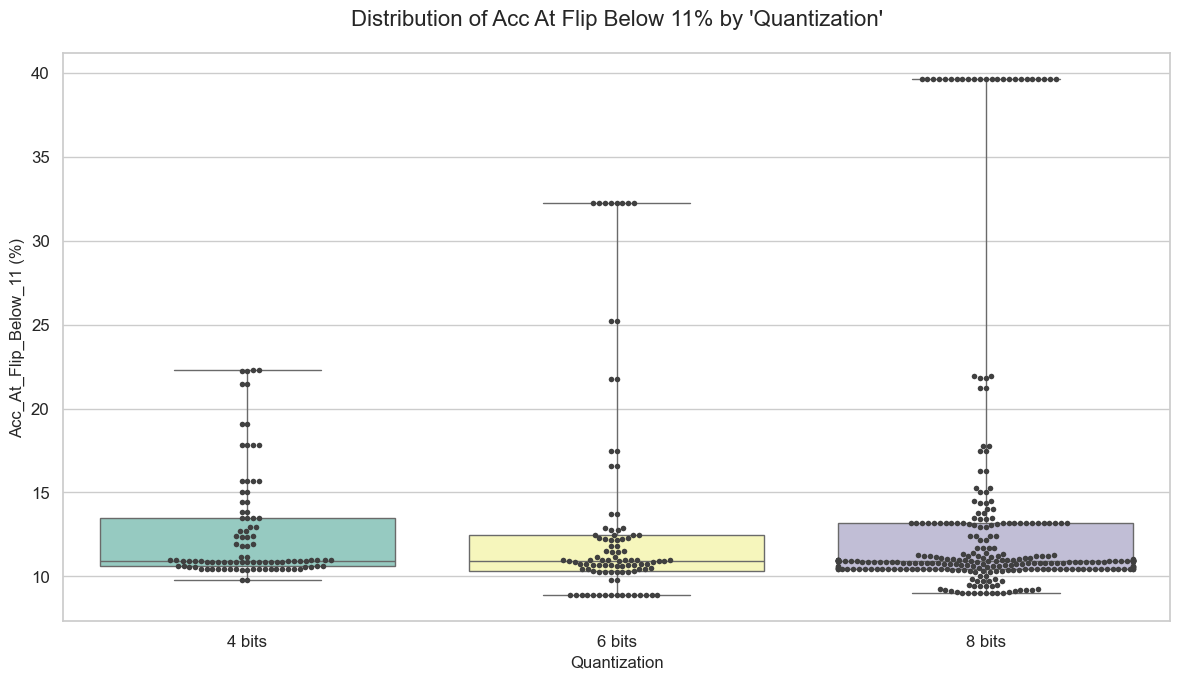
\includegraphics[width=0.5\textwidth]{Distribution of Acc Flip Below 11 by quantization.png}
    \caption{Distribution of final accuracy for successful attacks (target $<$ 11\%) by quantization level, aggregating results from all architectures and search algorithms.}
    \label{fig:quantization}
\end{figure}

\paragraph{Impact of Validation Set Size on Attack Efficiency}
\label{par:impacto_validacao}

To assess if a smaller validation set could accelerate the attack search without compromising effectiveness, we measured the impact of bit-flips using three set sizes:$1024, 2024, 10000$ samples. The statistical results from 482 attack runs for each configuration, presented in Table~\ref{tab:stats_validacao}, reveal a remarkable consistency. While the standard deviation is notable, measures of central tendency are extremely close. The mean final accuracy varied minimally (from 12.65\% to 13.50\%), and the median—a more robust metric—remained stable around 10.5\%--10.9\% for all configurations.

Figure~\ref{fig:impacto_validacao} provides visual confirmation, showing that the medians for the three validation set sizes are practically identical in the boxplot. The clear conclusion is that a large validation set does not yield a more effective attack. A smaller set of 1024 samples offers a statistically equivalent outcome but with a drastically reduced computational cost. This reduction cuts the number of inferences per fault evaluation by nearly 90\% compared to the 10000-sample set, making the PBS and EBS search processes significantly faster and more feasible.

% Troque TODO o ambiente tabular da Tabela IV por este:

\begin{table}[ht]
\centering
\scriptsize
\caption{Final accuracy statistics (\%) by validation set size over 482 runs. The proximity of mean and median values indicates that set size has a marginal impact on attack effectiveness.}
\label{tab:stats_validacao}

% Garante números alinhados e sem separador de milhar
\sisetup{
  group-separator = {},      % remove separador de milhar
  table-number-alignment = right
}

\begin{tabular}{
  S[table-format=5.0]  % Set Size (inteiro, alinhado à direita)
  S[table-format=2.2]  % Mean
  S[table-format=2.2]  % Median
  S[table-format=2.2]  % Std Dev
  S[table-format=2.2]  % IQR
}
\toprule
{\textit{Set Size (samples)}} & {\textit{Mean}} & {\textit{Median}} & {\textit{Std Dev}} & {\textit{IQR}} \\
\midrule
1024  & 13.22 & 10.68 & 8.56 & 1.49 \\
2024  & 12.65 & 10.89 & 6.62 & 2.83 \\
10000 & 13.50 & 10.51 & 8.43 & 3.16 \\
\bottomrule
\end{tabular}
\end{table}



\begin{figure}[htbp]
    \centering
    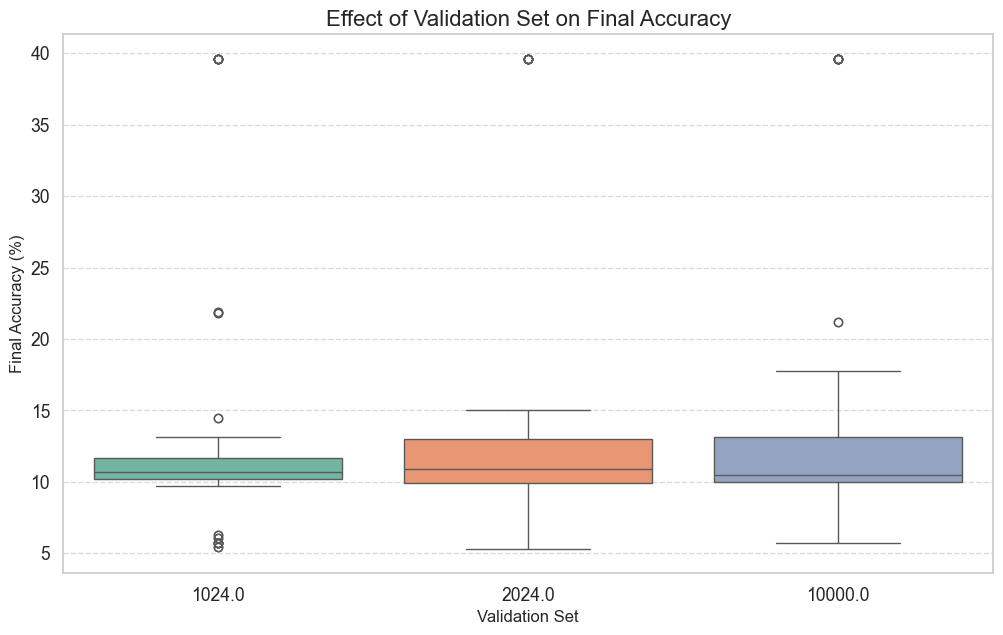
\includegraphics[width=0.5\textwidth]{effect_validation.png}
    \caption{Visual analysis of the effect of validation set size on the final post-attack accuracy. The boxplot compares the distributions for the three set sizes, showing that the medians are nearly identical, which validates the conclusion that a smaller set is sufficient.}
    \label{fig:impacto_validacao}
\end{figure}

\begin{table}[htbp]
    \centering
    \caption{Comparison of the minimum number of bit-flips ($N_{flips}$) between our method (MLBFA) and the state-of-the-art (Rakin et al.~\cite{Rakin2019}). Reference values are the median of 5 trials.}
    \label{tab:comparacao_sota_resize}
    \resizebox{\columnwidth}{!}{%
    \begin{tabular}{l c c c}
        \toprule
        \textit{Architecture} & \textit{Quant. (bits)} & \textit{$N_{flips}$ (Rakin et al.~\cite{Rakin2019})} & \textit{$N_{flips}$ (MLBFA)} \\
        \midrule
        \multirow{3}{*}{ResNet-20} & 8 & 11 & \textbf{9} \\
        & 6 & 10 & \textbf{9} \\
        & 4 & 8  & 9 \\
        \cmidrule(lr){2-4}
        \multirow{3}{*}{ResNet-32} & 8 & 14 & \textbf{6} \\
        & 6 & 13 & \textbf{6} \\
        & 4 & 13 & \textbf{6} \\
        \cmidrule(lr){2-4}
        \multirow{3}{*}{ResNet-44} & 8 & 12 & \textbf{10} \\
        & 6 & 15 & \textbf{12} \\
        & 4 & 22 & \textbf{11} \\
        \cmidrule(lr){2-4}
        \multirow{3}{*}{ResNet-56} & 8 & 19 & \textbf{10} \\
        & 6 & 18 & \textbf{11} \\
        & 4 & 20 & \textbf{10} \\
        \bottomrule
    \end{tabular}%
    }
\end{table}



% --- INSERIR ISTO NO FINAL DA SEÇÃO ANTERIOR (antes do \subsection novo) ---

% Tabela 1: Best-case comparison (Coluna única, força topo)
\begin{table}[!t]
    \centering
    \caption{Best-case comparison: Minimum number of bit-flips ($N_{flips}$) required to degrade accuracy below 11\%. We compare the standard MLBFA against our optimized MLBFA-Pruned method.}
    \label{tab:best_case_mlbfa_vs_pruned}
    \resizebox{\columnwidth}{!}{%
    \begin{tabular}{l c c c}
        \toprule
        \textit{Architecture} & \textit{Quant. (bits)} &
        \textit{$N_{flips}$ (MLBFA Standard)} &
        \textit{$N_{flips}$ (\textbf{MLBFA-Pruned})} \\
        \midrule
        \multirow{3}{*}{ResNet-20} & 8 & 9 & \textbf{7} \\
                                   & 6 & 9 & \textbf{8} \\
                                   & 4 & \textbf{9} & 11 \\
        \cmidrule(lr){2-4}
        \multirow{3}{*}{ResNet-32} & 8 & 6 & \textbf{4} \\
                                   & 6 & 6 & \textbf{4} \\
                                   & 4 & \textbf{6} & \textbf{6} \\
        \cmidrule(lr){2-4}
        \multirow{3}{*}{ResNet-44} & 8 & 10 & \textbf{9} \\
                                   & 6 & 12 & \textbf{11} \\
                                   & 4 & 11 & \textbf{8} \\
        \cmidrule(lr){2-4}
        \multirow{3}{*}{ResNet-56} & 8 & 10 & \textbf{5} \\
                                   & 6 & 11 & \textbf{6} \\
                                   & 4 & 10 & \textbf{7} \\
        \bottomrule
    \end{tabular}%
    }
\end{table}

% Tabela 2: Comparação SOTA Mediana (Coluna única, força topo)
\begin{table}[!t]
    \centering
    \caption{Comparison of the minimum number of bit-flips ($N_{flips}$) between the state-of-the-art (Rakin et al.~\cite{Rakin2019}) and our method (MLBFA-Pruned). The values for MLBFA-Pruned represent the median of successful attacks.}
    \label{tab:comparacao_sota_resize_mlbfa_pruned}
    \resizebox{\columnwidth}{!}{%
    \begin{tabular}{l c c c}
        \toprule
        \textit{Architecture} & \textit{Quant. (bits)} &
        \textit{$N_{flips}$ (Rakin et al.~\cite{Rakin2019})} &
        \textit{$N_{flips}$ (\textbf{MLBFA-Pruned})} \\
        \midrule
        \multirow{3}{*}{ResNet-20} & 8 & 11 & \textbf{9} \\
                                   & 6 & 10 & \textbf{8} \\
                                   & 4 & \textbf{8} & 11 \\
        \cmidrule(lr){2-4}
        \multirow{3}{*}{ResNet-32} & 8 & 14 & \textbf{6} \\
                                   & 6 & 13 & \textbf{5} \\
                                   & 4 & 13 & \textbf{6} \\
        \cmidrule(lr){2-4}
        \multirow{3}{*}{ResNet-44} & 8 & 12 & 12 \\
                                   & 6 & 15 & \textbf{13} \\
                                   & 4 & 22 & \textbf{11} \\
        \cmidrule(lr){2-4}
        \multirow{3}{*}{ResNet-56} & 8 & 19 & \textbf{9} \\
                                   & 6 & 18 & \textbf{9} \\
                                   & 4 & 20 & \textbf{12} \\
        \bottomrule
    \end{tabular}%
    }
\end{table}

% Tabela 3: Most efficient scenarios (Coluna dupla - automaticamente vai pro topo)
\begin{table*}[!t]
    \centering
    \caption{Most efficient attack scenarios for MLBFA-Pruned (accuracy $<$ 11\%): Minimum number of bit-flips ($N_{flips}$) required to degrade the network. Beta values refer to the VM that guided the respective attack. EBS denotes the evolutionary-based search (AG), and GBS denotes the greedy-based search.}
    \label{tab:best_attack_cases_mlbfa_pruned}
    \resizebox{0.77\textwidth}{!}{%
    \sisetup{group-separator = {}, table-number-alignment = right}
    \begin{tabular}{
        l % Architecture
        S[table-format=1.0, table-space-text-post = ~bits, table-text-post = ~bits] % Quantization
        l % Search Algorithm
        r % N_flips
        S[table-format=2.2] % Final Accuracy
        S[table-format=1.1] % Beta
    }
        \toprule
        \textit{Architecture} & \textit{Quantization} & \textit{Search Algorithm} &
        {\textit{$N_{flips}$}} & {\textit{Final Accuracy (\%)}} &
        {\textit{Beta (F-score)}} \\
        \midrule
        \multirow{3}{*}{ResNet-20} & 4 & GBS                  & 11 & 10.91 & 1.0 \\
                                   & 6 & \multirow{2}{*}{EBS} &  8 & 10.55 & 0.5 \\
                                   & 8 &                      &  7 & 10.45 & 1.0 \\
        \midrule
        \multirow{3}{*}{ResNet-32} & 4 & \multirow{2}{*}{GBS} &  6 & 10.25 & 0.5 \\
                                   & 6 &                      &  4 & 10.93 & 0.5 \\
                                   & 8 & EBS                  &  4 & 10.73 & 1.0 \\
        \midrule
        \multirow{3}{*}{ResNet-44} & 4 & \multirow{3}{*}{GBS} &  8 & 10.11 & 3.0 \\
                                   & 6 &                      & 11 & 10.68 & 2.3 \\
                                   & 8 &                      &  9 & 10.68 & 1.0 \\
        \midrule
        \multirow{3}{*}{ResNet-56} & 4 & \multirow{3}{*}{EBS} &  7 & 10.43 & 0.5 \\
                                   & 6 &                      &  6 & 10.79 & 2.3 \\
                                   & 8 &                      &  5 & 10.60 & 3.0 \\
        \bottomrule
    \end{tabular}%
    }
\end{table*}

% Tabela 4: Statistical Comparison (Coluna dupla - automaticamente vai pro topo)
\begin{table*}[!t]
    \centering
    \caption{Statistical comparison of the number of bit-flips ($N_{flips}$) between Rakin et al. (fixed 5 runs) and MLBFA-Pruned (variable runs). We report the Best (Minimum), Range (Min--Max), and Standard Deviation (Std Dev). The 'Runs' column denotes the total number of experimental trials performed for MLBFA-Pruned.}
    \label{tab:stat_comparison}
    \begin{tabular}{cc ccc cccc}
        \toprule
        & & \multicolumn{3}{c}{Rakin et al. \cite{Rakin2019}} & \multicolumn{4}{c}{MLBFA-Pruned (Ours)} \\
        \cmidrule(lr){3-5} \cmidrule(lr){6-9}
        Architecture & Bits & Best & Range & Std Dev & Runs & Best & Range & Std Dev \\
        \midrule
        \multirow{3}{*}{ResNet-20} & 8 & \textbf{7} & 7--17 & 3.70 & 24 & \textbf{7} & 7--14 & 2.29 \\
         & 6 & \textbf{8} & 8--13 & 2.30 & 8 & \textbf{8} & 8--13 & 2.24 \\
         & 4 & \textbf{7} & 7--12 & 2.17 & 8 & 11 & 11--11 & 0.00 \\
        \cmidrule(lr){1-9}
        \multirow{3}{*}{ResNet-32} & 8 & 8 & 8--31 & 9.40 & 24 & \textbf{4} & 4--11 & 2.28 \\
         & 6 & 9 & 9--23 & 5.59 & 8 & \textbf{4} & 4--7 & 1.00 \\
         & 4 & 10 & 10--17 & 2.61 & 8 & \textbf{6} & 6--6 & 0.00 \\
        \cmidrule(lr){1-9}
        \multirow{3}{*}{ResNet-44} & 8 & \textbf{6} & 6--22 & 5.94 & 24 & 9 & 9--21 & 3.50 \\
         & 6 & 13 & 13--17 & 1.79 & 8 & \textbf{11} & 11--16 & 2.52 \\
         & 4 & 14 & 14--50 & 15.79 & 8 & \textbf{8} & 8--14 & 2.34 \\
        \cmidrule(lr){1-9}
        \multirow{3}{*}{ResNet-56} & 8 & 16 & 16--22 & 2.83 & 24 & \textbf{5} & 5--12 & 1.89 \\
         & 6 & 16 & 16--21 & 2.35 & 8 & \textbf{6} & 6--10 & 1.37 \\
         & 4 & 9 & 9--24 & 6.07 & 8 & \textbf{7} & 7--17 & 4.11 \\
        \bottomrule
    \end{tabular}
\end{table*}



\subsection{Analysis of BFA Efficiency}
\label{subsec:analise_bfa}

Armed with a high-quality ranking provided by the VM, we evaluated the effectiveness of each BFA search algorithm. The central objective was to determine the minimum number of bit-flips ($N_{flips}$) required to induce a catastrophic network failure, defined as the degradation of accuracy to a level below 11\%. Table~\ref{tab:best_attack_cases} summarizes the results of the most efficient attacks for each architecture and quantization combination, highlighting the best-performing search algorithm and the characteristics of the VM that guided it.

The results underscore the high efficacy of the MLBFA framework, which neutralized target models with a minimal number of faults. In an emblematic case, the \textit{ResNet-32} architecture was compromised by just 6 bit-flips across all tested precisions (4, 6, and 8 bits). To contextualize this performance, we benchmarked our method against the "Bit-Flip Attack" by Rakin et al.~\cite{Rakin2019}, a key reference for quantized ResNet attacks on the CIFAR-10 dataset. The comparison in Table~\ref{tab:comparacao_sota_resize} shows that our framework surpasses this baseline, particularly for deeper models; for \textit{ResNet-56}, it required approximately half the bit-flips to achieve model failure (e.g., 10 vs. 20 at 4-bit precision). This advantage substantiates our core hypothesis: guiding an attack via ML-based vulnerability prediction is more strategic than a search based on gradients alone. While the conventional approach uses a single metric, our VM leverages a multi-dimensional feature vector to discern intricate, non-linear patterns, leading to its superior performance.

A comparative analysis of our own search algorithms, based on the data in Table~\ref{tab:best_attack_cases}, reveals clear performance patterns. The EBS, based on a Genetic Algorithm, proved to be the dominant strategy for shallower architectures, winning in all scenarios for ResNet-20 and ResNet-32. Its ability to explore synergistic combinations of flips was crucial in these networks. In contrast, the GBS, our greedy search implementation, proved more effective in the deeper architectures, winning in most scenarios for ResNet-56.


% --- INSERIR ANTES DA SUBSECTION ---

% Tabela Grande (GA vs GBS - Regressão)
% Tabela Grande (Horizontal) - Performance da Regressão
\begin{table*}[!t]
    \centering
    \caption{Performance comparison of Regression-based vulnerability ranking using different SFI paradigms (BIT-ITER, BIT-ONE, LAYER, NET) for training data generation. The table compares Genetic Algorithm (GA) vs. Greedy Bit Search (GBS), split side-by-side: ResNet-20/32 (Left) and ResNet-44/56 (Right).}
    \label{tab:comparison_regression_horizontal}
    \scriptsize % Fonte menor
    \setlength{\tabcolsep}{3pt} % Espaçamento reduzido
    \begin{tabular}{cc ccc ccc | cc ccc ccc}
        \toprule
        & & \multicolumn{3}{c}{\textbf{GA}} & \multicolumn{3}{c|}{\textbf{GBS}} & 
        & & \multicolumn{3}{c}{\textbf{GA}} & \multicolumn{3}{c}{\textbf{GBS}} \\
        \cmidrule(lr){3-5} \cmidrule(lr){6-8} \cmidrule(lr){11-13} \cmidrule(lr){14-16}
        
        Err & SFI & Bits & Acc. & Rch & Bits & Acc. & Rch & 
        Err & SFI & Bits & Acc. & Rch & Bits & Acc. & Rch \\
        \midrule
        
        % ResNet-20 vs ResNet-44
        \multicolumn{8}{c|}{\textbf{ResNet-20}} & \multicolumn{8}{c}{\textbf{ResNet-44}} \\
        \midrule
        0.5\% & BIT-ITER & 8 & 0.1094 & Yes & 8 & 0.1025 & Yes & 0.5\% & BIT-ITER & 12 & 0.6074 & No & 120 & 0.5869 & No \\
        0.5\% & BIT-ONE & 9 & 0.1895 & No & 8 & 0.1025 & Yes & 0.5\% & BIT-ONE & 11 & 0.2803 & No & 120 & 0.7852 & No \\
        0.5\% & LAYER & 9 & 0.1221 & No & 12 & 0.1035 & Yes & 0.5\% & LAYER & 12 & 0.1934 & No & 36 & 0.1094 & Yes \\
        0.5\% & NET & 7 & 0.1094 & Yes & 9 & 0.1064 & Yes & 0.5\% & NET & 3 & 0.8125 & No & 120 & 0.8994 & No \\
        \cmidrule{1-16}
        1\% & BIT-ITER & 6 & 0.8652 & No & 120 & 0.8125 & No & 1\% & BIT-ITER & 1 & 0.9023 & No & 120 & 0.9004 & No \\
        1\% & BIT-ONE & 9 & 0.1162 & No & 9 & 0.1064 & Yes & 1\% & BIT-ONE & 12 & 0.2734 & No & 47 & 0.1094 & Yes \\
        1\% & LAYER & 9 & 0.1514 & No & 10 & 0.1064 & Yes & 1\% & LAYER & 12 & 0.3027 & No & 120 & 0.1611 & No \\
        1\% & NET & 9 & 0.1982 & No & 24 & 0.1094 & Yes & 1\% & NET & 12 & 0.5117 & No & 120 & 0.7295 & No \\
        \cmidrule{1-16}
        5\% & BIT-ITER & 1 & 0.8994 & No & 120 & 0.8838 & No & 5\% & BIT-ITER & 2 & 0.9004 & No & 120 & 0.8135 & No \\
        5\% & BIT-ONE & 9 & 0.2236 & No & 120 & 0.1738 & No & 5\% & BIT-ONE & 12 & 0.3037 & No & 120 & 0.3174 & No \\
        5\% & LAYER & 9 & 0.2715 & No & 45 & 0.1084 & Yes & 5\% & LAYER & 12 & 0.2832 & No & 120 & 0.1670 & No \\
        5\% & NET & 1 & 0.9053 & No & 120 & 0.9053 & No & 5\% & NET & 1 & 0.9023 & No & 120 & 0.9023 & No \\
        
        \midrule
        % ResNet-32 vs ResNet-56
        \multicolumn{8}{c|}{\textbf{ResNet-32}} & \multicolumn{8}{c}{\textbf{ResNet-56}} \\
        \midrule
        0.5\% & BIT-ITER & 6 & 0.2266 & No & 15 & 0.1074 & Yes & 0.5\% & BIT-ITER & 10 & 0.3467 & No & 120 & 0.2178 & No \\
        0.5\% & BIT-ONE & 6 & 0.3838 & No & 33 & 0.1094 & Yes & 0.5\% & BIT-ONE & 8 & 0.3125 & No & 120 & 0.4053 & No \\
        0.5\% & LAYER & 6 & 0.3604 & No & 29 & 0.1094 & Yes & 0.5\% & LAYER & 10 & 0.1602 & No & 32 & 0.1094 & Yes \\
        0.5\% & NET & 6 & 0.3799 & No & 120 & 0.6348 & No & 0.5\% & NET & 1 & 0.9131 & No & 120 & 0.9131 & No \\
        \cmidrule{1-16}
        1\% & BIT-ITER & 6 & 0.5791 & No & 120 & 0.5752 & No & 1\% & BIT-ITER & 9 & 0.1064 & Yes & 10 & 0.0928 & Yes \\
        1\% & BIT-ONE & 6 & 0.1143 & No & 11 & 0.1094 & Yes & 1\% & BIT-ONE & 10 & 0.2549 & No & 120 & 0.1865 & No \\
        1\% & LAYER & 6 & 0.1523 & No & 23 & 0.1094 & Yes & 1\% & LAYER & 10 & 0.2080 & No & 29 & 0.1094 & Yes \\
        1\% & NET & 1 & 0.8994 & No & 120 & 0.9053 & No & 1\% & NET & 5 & 0.8828 & No & 120 & 0.8457 & No \\
        \cmidrule{1-16}
        5\% & BIT-ITER & 1 & 0.8975 & No & 120 & 0.9004 & No & 5\% & BIT-ITER & 1 & 0.9131 & No & 120 & 0.9131 & No \\
        5\% & BIT-ONE & 6 & 0.1279 & No & 10 & 0.1035 & Yes & 5\% & BIT-ONE & 9 & 0.2734 & No & 120 & 0.2275 & No \\
        5\% & LAYER & 6 & 0.3535 & No & 120 & 0.1494 & No & 5\% & LAYER & 10 & 0.2520 & No & 27 & 0.1094 & Yes \\
        5\% & NET & 1 & 0.8994 & No & 120 & 0.8994 & No & 5\% & NET & 10 & 0.3262 & No & 120 & 0.4307 & No \\
        \bottomrule
    \end{tabular}
\end{table*}

% Tabela Resumo Vertical
\begin{table}[!t]
    \centering
    \caption{Best attack scenarios for Regression-based ranking per architecture. Configuration format: Algorithm / SFI Paradigm (Target Error).}
    \label{tab:best_case_regression}
    \resizebox{\columnwidth}{!}{%
    \begin{tabular}{llcc}
        \toprule
        Architecture & Configuration & Bits & Final Acc. \\
        \midrule
        ResNet-20 & EBS / NET (0.5\%) & 7 & 0.1094 \\
        ResNet-32 & GBS / BIT-ONE (5\%) & 10 & 0.1035 \\
        ResNet-44 & GBS / LAYER (0.5\%) & 36 & 0.1094 \\
        ResNet-56 & EBS / BIT-ITER (1\%) & 9 & 0.1064 \\
        \bottomrule
    \end{tabular}%
    }
\end{table}







\subsection{Extended Analysis: Pruning Efficiency and Statistical Comparison}
\label{subsec:extended_analysis}

Building upon the initial BFA efficiency analysis, we assessed the impact of integrating a pruning mechanism (MLBFA-Pruned) into our framework. The primary goal was to determine if reducing the search space via pruning could further minimize the fault injection cost required to degrade accuracy below 11\%. Table~\ref{tab:best_case_mlbfa_vs_pruned} offers a direct comparison between the standard MLBFA and its pruned variant. The data reveals that the pruning strategy significantly enhances attack efficiency, particularly in deeper architectures. For instance, in the 8-bit \textit{ResNet-56} model, the pruned variant reduced the required bit-flips from 10 to 5, achieving a 50\% reduction compared to the standard approach. Overall, MLBFA-Pruned outperformed or matched the standard version in 11 out of 12 experimental configurations, validating the hypothesis that a targeted search space leads to more economical attacks.

Table~\ref{tab:best_attack_cases_mlbfa_pruned} summarizes the most efficient attack scenarios discovered by MLBFA-Pruned. A comparative analysis of the search algorithms reveals a distinct trade-off: while the Greedy-Based Search (GBS) proved effective for intermediate depths (e.g., \textit{ResNet-44}), the Evolutionary-Based Search (EBS) demonstrated superior performance in the deepest architecture (\textit{ResNet-56}). This suggests that genetic algorithms are better suited to navigate the complex, non-linear search landscapes of deeper, pruned networks, where finding synergistic fault combinations is critical.

To rigorously benchmark our optimized method, we compared our results against Rakin et al.~\cite{Rakin2019}, a leading state-of-the-art BFA method. While Table~\ref{tab:comparacao_sota_resize_mlbfa_pruned} provides an overview using median values—where MLBFA-Pruned already shows a clear advantage—a more robust statistical assessment is presented in Table~\ref{tab:stat_comparison}. Unlike the baseline, which reports the best result over 5 trials, we validated our approach with a significantly larger sample size (up to 24 runs per configuration) to ensure statistical reliability.

The comprehensive comparison in Table~\ref{tab:stat_comparison} confirms the superiority of our method. MLBFA-Pruned achieves a lower or equal number of bit-flips in 10 out of 12 configurations when comparing absolute best cases. The advantage is most pronounced in deeper models; for \textit{ResNet-56} at 8-bit precision, our method requires only 5 flips compared to the 16 reported by the baseline. Furthermore, the lower standard deviation observed across our extensive trials indicates not only higher efficiency but also greater stability and reproducibility of the attacks generated by the MLBFA-Pruned framework.




% --- INÍCIO DA SUBSECTION ---

\subsection{Evaluation of Regression-Based Vulnerability Ranking}
\label{subsec:regression_analysis}

Complementing the classification-based analysis, we investigated an alternative regression-based strategy, where the VM is trained to predict the exact magnitude of accuracy degradation caused by a bit-flip. Table~\ref{tab:comparison_regression_horizontal} details the performance of the Genetic Algorithm (GA) and Greedy Bit Search (GBS) under this guidance. Crucially, the ``SFI Paradigm'' column indicates the source of the training data—\textit{Bit-Wise} (BIT-ONE, BIT-ITER) or coarser structural approaches (LAYER, NET)—allowing us to assess how data granularity influences the quality of the regression.

A critical comparison with the classification results in Section~\ref{subsec:extended_analysis} reveals that regression-based ranking yields significantly less efficient attacks. As summarized in Table~\ref{tab:best_case_regression}, the computational cost to degrade the network increased considerably across nearly all architectures. For instance, in \textit{ResNet-32}, the most efficient regression attack (guided by a VM trained on BIT-ONE data) required 10 bit-flips, whereas the classification approach achieved the same goal with only 4 flips. This performance gap widens in deeper networks: for \textit{ResNet-44}, the regression method struggled to converge, necessitating 36 flips in the best-case scenario (using LAYER data), compared to just 8 flips with classification. Even in \textit{ResNet-56}, where the Evolutionary-Based Search (EBS) found a viable solution with 9 flips (using BIT-ITER data), it remained inferior to the 5 flips achieved by the classification model.

The data in Table~\ref{tab:comparison_regression_horizontal} further highlights stability issues inherent to the regression approach. A substantial number of GA runs failed to reach the target accuracy (indicated by ``No'' in the \textit{Reached} column), particularly in deeper architectures. This suggests that the regression signal—attempting to map structural features to a continuous, noisy error value—lacks the clear decision boundaries provided by the classification model. While the GBS demonstrated a higher success rate in finding valid solutions (e.g., in ResNet-44 where GA failed), it often required a disproportionately higher number of flips. This indicates that the gradients provided by the regression VM, even when trained with high-fidelity paradigms like BIT-ONE, were suboptimal for efficiently guiding the search toward the most critical bits. Consequently, predicting the exact impact of a fault introduces unnecessary complexity; the binary classification approach proves to be a more robust and effective signal for adversarial fault injection.

\section{Conclusion}
\label{sec:conclusions}

This work introduced MLBFA, a framework that integrates machine learning with statistical fault injection to conduct highly efficient Bit-Flip Attacks. By leveraging a multidimensional feature set and integrating a novel search pruning mechanism (MLBFA-Pruned), our approach outperformed state-of-the-art gradient-based methods. Supported by extensive statistical validation across up to 24 trials per configuration, our method neutralized a ResNet-32 with as few as four bit-flips and reduced the required flips by nearly 70\% on deeper models like the ResNet-56 compared to the standard approach.

Our analysis also yielded crucial insights into ML-guided attack dynamics. We established that framing vulnerability prediction as a binary classification task provides a significantly more robust signal than regression-based ranking, which proved computationally inefficient and unstable in our experiments. We found the optimal VM to be highly scenario-dependent, showing that a single Precision-Recall trade-off is not universally applicable, which in turn determined the best-performing search algorithm for a given network depth. Furthermore, our results across 4, 6, and 8-bit models showed that while the attacks were consistently effective in neutralizing the networks, models with higher precision occasionally exhibited greater residual robustness post-attack. This investigation was made practical by our finding that a small validation set is sufficient for evaluating fault impact in the initial SFI campaign, drastically cutting the computational costs of this first stage by nearly 90\%.

Future work will extend the framework to new architectures and targeted attacks, expand the fault model to Multiple Bit-Upsets (MBUs), and use its vulnerability maps to guide selective hardware protection schemes, such as error-correcting codes (ECC).

\begin{thebibliography}{00}

\bibitem{Lin}
C. S. Lin, J. Qu, and G. Saileshwar, ``GPUHammer: Rowhammer attacks on GPU memories are practical,'' arXiv [cs.CR], 2025.

\bibitem{indi}
Global Desk, ``Nvidia chips hacked, fall victim to Rowhammer bit-flip attacks; here’s how to secure the AI GPUs,'' \textit{The Economic Times}, Jul. 16, 2025. [Online]. Available: (URL). Accessed: Jul. 26, 2025.

\bibitem{Qian2023}
C. Qian, M. Zhang, Y. Nie, S. Lu, and H. Cao, ``A survey of bit-flip attacks on deep neural network and corresponding defense methods,'' \textit{Electronics}, vol. 12, no. 4, p. 853, 2023.

\bibitem{Kim2014}
Y. Kim \textit{et al.}, ``Flipping bits in memory without accessing them: An experimental study of DRAM disturbance errors,'' \textit{ACM SIGARCH Comput. Archit. News}, vol. 42, no. 3, pp. 361--372, 2014.

\bibitem{BREIER2023}
J. Breier and X. Hou, ``How practical are fault injection attacks, really?'' \textit{IEEE Access}, vol. 10, pp. 113122--113130, 2022.

\bibitem{bosio2019}
A. Bosio, P. Bernardi, A. Ruospo, and E. Sanchez, ``A reliability analysis of a deep neural network,'' in \textit{Proc. 2019 IEEE Latin American Test Symp. (LATS)}, 2019, pp. 1--6.

\bibitem{ruospo2020}
A. Ruospo, A. Bosio, A. Ianne, and E. Sanchez, ``Evaluating convolutional neural networks reliability depending on their data representation,'' in \textit{Proc. 2020 23rd Euromicro Conf. Digital Syst. Design (DSD)}, 2020, pp. 672--679.

\bibitem{Ahmadilivani2024}
M. H. Ahmadilivani, M. Taheri, J. Raik, M. Daneshtalab, and M. Jenihhin, ``A systematic literature review on hardware reliability assessment methods for deep neural networks,'' \textit{ACM Comput. Surv.}, vol. 56, no. 6, pp. 1--39, Art. 141, Jan. 2024.

\bibitem{Liu2017}
Y. Liu, L. Wei, B. Luo, and Q. Xu, ``Fault injection attack on deep neural network,'' in \textit{Proc. 2017 IEEE/ACM Int. Conf. Comput.-Aided Design (ICCAD)}, 2017, pp. 131--138.

\bibitem{sabbagh2019evaluating}
M. Sabbagh, C. Gongye, Y. Fei, and Y. Wang, ``Evaluating fault resiliency of compressed deep neural networks,'' in \textit{Proc. 2019 IEEE Int. Conf. Embedded Softw. and Syst. (ICESS)}, 2019, pp. 1--7.

\bibitem{Torres}
C. Torres-Huitzil and B. Girau, ``Fault and error tolerance in neural networks: A review,'' \textit{IEEE Access}, vol. 5, pp. 17322--17341, 2017.

\bibitem{Yu}
G. Yu \textit{et al.}, ``A survey on failure analysis and fault injection in AI systems,'' \textit{ACM Trans. Softw. Eng. Methodol.}, May 2025.

\bibitem{Arlat1990}
J. Arlat, Y. Crouzet, and J. C. Laprie, ``Fault injection for dependability validation: A methodology and some applications,'' \textit{IEEE Trans. Softw. Eng.}, vol. 16, no. 2, pp. 166--182, Feb. 1990.

\bibitem{Ruospo2021}
A. Ruospo \textit{et al.}, ``Pros and cons of fault injection approaches for the reliability assessment of deep neural networks,'' in \textit{Proc. 2021 IEEE 22nd Latin American Test Symp. (LATS)}, 2021, pp. 1--5.

\bibitem{Ruospo2023}
A. Ruospo \textit{et al.}, ``A survey on deep learning resilience assessment methodologies,'' \textit{Computer}, vol. 56, no. 2, pp. 57--66, 2023.

\bibitem{Mahmoudetal2020}
A. Mahmoud \textit{et al.}, ``PyTorchFI: A runtime perturbation tool for DNNs,'' in \textit{Proc. 2020 50th Annu. IEEE/IFIP Int. Conf. Dependable Syst. and Netw. Workshops (DSN-W)}, 2020, pp. 25--31.

\bibitem{chen2018tensorfi}
Z. Chen \textit{et al.}, ``TensorFI: A flexible fault injection framework for TensorFlow applications,'' in \textit{Proc. 2020 IEEE 31st Int. Symp. Softw. Reliability Eng. (ISSRE)}, 2020, pp. 426--435.

\bibitem{Huang2023MRFI}
H. Huang, C. Liu, X. Xue, Y. Wang, H. Li, and X. Li, ``MRFI: An open source multi-resolution fault injection framework for neural network processing,'' arXiv, Jan. 2023.

\bibitem{Gavarini2023}
G. Gavarini, A. Ruospo, and E. Sanchez, ``A fast reliability analysis of image segmentation neural networks exploiting statistical fault injections,'' in \textit{Proc. 2023 IEEE 24th Latin American Test Symp. (LATS)}, 2023, pp. 1--6.

\bibitem{Zheng2023}
Y. Zheng, Z. Feng, Z. Hu, and K. Pei, ``MindFI: A fault injection tool for reliability assessment of MindSpore applications,'' in \textit{Proc. 2021 IEEE Int. Symp. Softw. Reliability Eng. Workshops (ISSREW)}, 2021, pp. 235--238.

\bibitem{Gogebakan}
A. B. Göğebakan, E. Magliano, A. Carpegna, A. Ruospo, A. Savino, and S. D. Carlo, ``SpikingJET: Enhancing fault injection for fully and convolutional spiking neural networks,'' arXiv, Jul. 2024.

\bibitem{reagen2018ares}
B. Reagen \textit{et al.}, ``ARES: A framework for quantifying the resilience of deep neural networks,'' in \textit{Proc. 2018 55th ACM/ESDA/IEEE Design Autom. Conf. (DAC)}, 2018, pp. 1--6.

\bibitem{agarwal_lltfi_2021}
U. K. Agarwal, A. Chan, and K. Pattabiraman, ``LLTFI: Framework-agnostic fault injection for machine learning applications,'' in \textit{Proc. 2022 IEEE Int. Symp. Softw. Reliability Eng. (ISSRE)}, 2022.


\bibitem{Zhang2023}
Y. Zhang, H. Itsuji, T. Uezono, T. Toba, and M. Hashimoto, ``Vulnerability estimation of DNN model parameters with few fault injections,'' \textit{IEICE Trans. Fundam. Electron. Commun. Comput. Sci.}, vol. E106-A, no. 3, pp. 523--530, 2023.

\bibitem{salih2022survey}
R. T. Syed, M. Ulbricht, K. Piotrowski, and M. Krstic, ``A survey on fault-tolerant methodologies for deep neural networks,'' \textit{Elektronika}, vol. 64, no. 2, pp. 89--98, 2023.

\bibitem{ruospo2023assessing}
A. Ruospo \textit{et al.}, ``Assessing convolutional neural networks reliability through statistical fault injections,'' in \textit{Proc. 2023 Design, Autom. \& Test in Europe Conf. \& Exhib. (DATE)}, 2023.

\bibitem{ruospo2025iterative}
A. Ruospo, M. S. Reorda, R. Mariani, and E. Sanchez, ``An effective iterative statistical fault injection methodology for deep neural networks,'' \textit{IEEE Trans. Comput.}, pp. 1--14, Jan. 2025.

\bibitem{Zhang2022}
Y. Zhang, H. Itsuji, T. Uezono, T. Toba, and M. Hashimoto, ``Estimating vulnerability of all model parameters in DNN with a small number of fault injections,'' in \textit{Proc. 2022 Design, Autom. \& Test in Europe Conf. \& Exhib. (DATE)}, 2022.


\bibitem{leveugle2009statistical}
R. Leveugle, A. Calvez, P. Maistri, and P. Vanhauwaert, ``Statistical fault injection: Quantified error and confidence,'' in \textit{Proc. 2009 Design, Autom. \& Test in Europe Conf. \& Exhib. (DATE)}, 2009, pp. 502--506.

\bibitem{Traiola2023hardnning}
M. Traiola, A. Kritikakou, and O. Sentieys, ``A machine-learning-guided framework for fault-tolerant DNNs,'' in \textit{Proc. Design, Autom. \& Test in Europe Conf. \& Exhib. (DATE)}, 2015, pp. 1--2, Apr. 2023.

\bibitem{harDNNing2023}
M. Traiola, A. Kritikakou, and O. Sentieys, ``harDNNing: A machine-learning-based framework for fault tolerance assessment and protection of DNNs,'' May 2023.

\bibitem{Huang2020Functional}
Y. Huang, P. H. Siegel, and A. Jiang, ``Functional error correction for robust neural networks,'' \textit{IEEE J. Sel. Areas Inf. Theory}, vol. 1, no. 2, pp. 445--457, 2020.

\bibitem{Rakin2019}
A. S. Rakin, Z. He, and D. Fan, ``Bit-flip attack: Crushing neural network with progressive bit search,'' in \textit{Proc. IEEE/CVF Int. Conf. Comput. Vis. (ICCV)}, 2019, pp. 1211--1220.

\bibitem{Rakin2021}
A. S. Rakin \textit{et al.}, ``T-BFA: Targeted bit-flip adversarial weight attack,'' \textit{IEEE Trans. Pattern Anal. Mach. Intell.}, vol. 44, no. 11, pp. 7928--7939, 2022.

\bibitem{Hector2022}
M. Dumont, J.-M. Dutertre, A.-P. Mirbaha, A. Tria, and H. L. Hector, ``A closer look at evaluating the bit-flip attack against deep neural networks,'' in \textit{Proc. 2022 IEEE Int. Workshop Inf. Forensics and Secur. (WIFS)}, 2022.

\bibitem{Dong}
J. Dong \textit{et al.}, ``One-bit flip is all you need: When bit-flip attack meets model training,'' in \textit{Proc. IEEE/CVF Int. Conf. Comput. Vis. (ICCV)}, 2023.

\end{thebibliography}


\vspace{12pt}
\end{document}
